%----------------------------------------------------------------
%
%  File    :  project-listmerger.tex
%
%  Author  :  Martin Rabensteiner
% 
%  Created :  20 Feb 2026
% 
%  Changed :  01 Jul 2026
% 
%----------------------------------------------------------------

\chapter{ListMerger}
\label{chap:listmerger}

This section describes implementation details of ListMerger. The code
itself is written in pure TypeScript. Almost all third-party libraries
are used only in the build and development process. Only the Mustache
package is used to render templates during runtime.

Recurring terms in the development are \uiname{move} and \uiname{merge}.
Moving describes the process of a transferring an item from an
\uiname{origin list} to the \uiname{mergelist}. A merged item always
consists of two predecessors. They are either taken from the mergelist
(merged or moved), or directly taken from the evaluators list. The
origin is always tracked, independent whether the item is coming from an
origin list or the mergelist. The differentiation between moved and
origin is done, to have a clean and reconstructive merging history.


\section{Architecture and Files}
The library itself is modularised into several TypeScript files and
compiled with Gulp to a single \fname{.js} file. Minimised and Gzip
files, as well as a CSS stylesheet are added. This stylesheet contains
the recommended minimum styling to build a proper example. The only
dependency at runtime is Mustache \parencite{mustache} to render
user-specific templates. The TypeScript files are:
\begin{itemize}
\item \fname{events.ts}: Initialises all event listeners for buttons and
drag events, and contains their functions.

\item \fname{globalvars.ts}: Contains some shared variables, all above
the data structure for lists and items during runtime.

\item \fname{history.ts}: Tracks all actions and recovers them when the
\uiname{Undo} or \uiname{Redo} button is pressed.

\item \fname{index.ts}: Serves as the interface between the module
and the outer implementation.

\item \fname{init.ts}: Contains the only function callable from the
outside.

\item \fname{transfer.ts}: Handles the transfers between the source
lists and the merged list.

\item \fname{uihelper.ts}: Contains several helper functions to deal
with the DOM.
\end{itemize}




\section{Initialisation and Data Structure}
An initialisation call is necessary to activate the functionality of the
library. For this, the function \vname{init.init()} is called from the
outside. More details on this call are described in
Section~\ref{sec:libu-init}. This function calls all necessary
initialising functions of all files.

When initialising, a JavaScript object has to be handed over to the
library in order to build the application. This object needs to contain
at least a \vname{merged} key and an \vname{originlists} key. More
details on this data structure can be found in
Section~\ref{sec:libu-datastructure}, with Listing~\ref{list:itemslist}
as example. The object is modified with every user action and is
returned with the \vname{getAllItems()} function.

ListMerger itself does not define its own style, but certain CSS
styling rules are highly recommended and can be found in
\fname{listmerger.css}.




\section{History (Undo/Redo)}
An important feature and affordance of this component is the history
tracking, to keep track of user actions. With the \uiname{Undo} and
\uiname{Redo} buttons, the user can jump back and forward with actions. 

The history is based on a history and a future array. When clicking
undo/redo, a history item is moved from history to future, or vice
versa. A history item consists of a keyword for the action, and several
parameters, to track IDs, positions, arrays and so on, depending on the
context of the merge keyword. User actions are tracked with the
\vname{history.log()} function.




\section{Tab Bar}

\begin{samepage}
\begin{lstlisting}[%
float=tp,
aboveskip=\floatsep,
belowskip=\floatsep,
xleftmargin=0cm,              % no extra margins for floats
xrightmargin=0cm,             % no extra margins for floats
basicstyle=\footnotesize\ttfamily,
frame=shadowbox,
numbers=left,
language=CSS,
label=list:tabbarcss,
caption={[Tab Bar CSS]%
The minimal CSS styling to use the \elname{details} element and its
children as a tab bar.
},
]
.container {
  display: flex;
  flex-wrap: wrap;
}

details {
  display: contents;
}

details[open]::details-content {
  display: contents;
}

summary {
  order: 0;
}

section {
  order: 1;
  width: 100%;
}
\end{lstlisting}
\end{samepage}


For a long time, it was necessary to use JavaScript event listeners for
tab bars in the web. By adding click event listeners to the title, the
appearance of the content below in that way can be controlled. The
\elname{details} HTML element and some CSS adjustments make it possible
to have tab bars without JavaScript.

The \elname{details} element serves as a container for one item. On
\elname{summary} element is needed as a child, which is represents the
title. If no such title element is present, the total is
\uiname{Details}. Per default, a small triangle on the left indicates
the open/closed status of the content. This status is toggled by
clicking on the \elname{summary} element. The content does not
necessarly have to be an element and can also be plain text. To have a
clear structure, it is still advisable to have an element to give the
content a better structure, for example with a \elname{section} element.
With the \vname{open} attribute, the fold out of \elname{details} can be
controlled. The \vname{name} attribute can be used to only open one
\elname{details} box when having several instances.

The original purpose of this element is to build Accordions. To use it
for tab bars, some CSS properties need to be applied. These properties
include:
\begin{itemize}
\item \liintro{\elname{container} as flexbox}: This ensure to have the
elements next to each in horizontal alignment.

\item \liintro{\elname{section} with full-width (100\%)}: Below the flex
container, the summaries should have only as much width as they need,
but the section below should span across the whole width to break in a
new line.

\item \liintro{Display details as content}: The section would be shown
right next to the summary, but this display option shifts it to the end.

\item \liintro{Display open details pseudo-element as content}: This
pseudo element 

\item \liintro{Order of summary and section}: Setting the order for all
summary items to 0 and all section items to 1, clusters the summary
items all at the top and shows the active section element below.
\end{itemize}

The minimal CSS to reach this appearance in shown in
Listing~\ref{list:tabbarcss}. Additionally, the tabs are also styled
with some basic CSS, including, colours, borders, border rounding,
margins, paddings, and the cursor to reach a familiar visual appearance,
as seen in Figure~\ref{fig:tabs}.

\begin{figure}[tp]
\centering
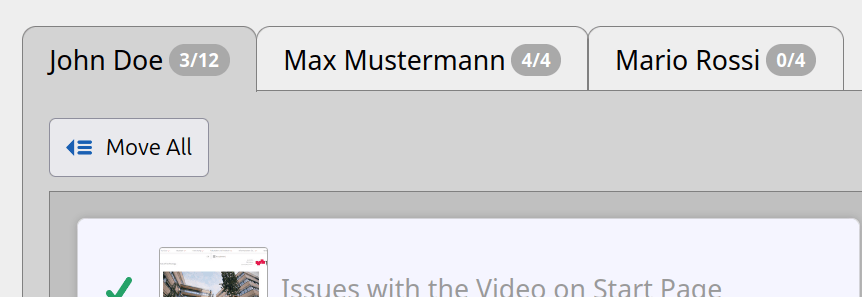
\includegraphics[frame,keepaspectratio,width=\halfh,height=\thirdh]
{images/tabs-i.png}
\caption[Tabs]{%
The tabs in ListMerger show the title of each list and an indicator with
the number of added/merged and total items in the list.
\imgcredit{Screenshot by Martin Rabensteiner.}
}
\label{fig:tabs}
\end{figure}

\begin{figure}[tp]
\centering
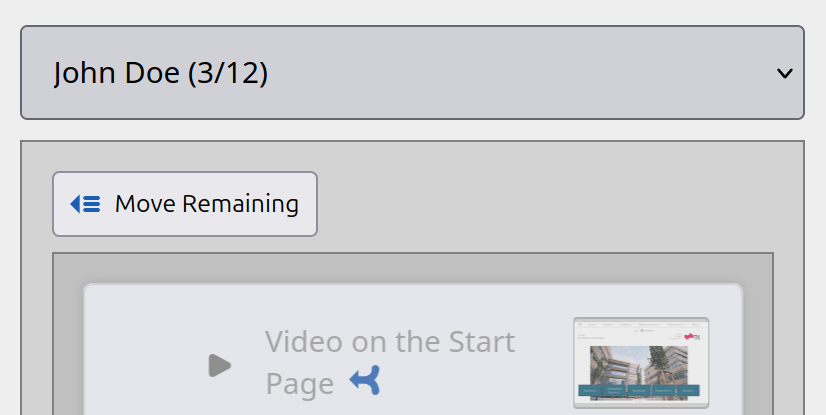
\includegraphics[frame,keepaspectratio,width=\halfh,height=\quarterh]
{images/tab-compact-i.png}
\caption[Tabs Select Box]{%
With less space, tabs are condensed into a select box.
\imgcredit{Screenshot by Martin Rabensteiner.}
}
\label{fig:tabs-compact}
\end{figure}



% Responsive Tabbar
However, to maintain responsiveness the solution in ListMerger still
uses JavaScript to transform the bar of tabs into a selection box on
smaller screens, or with longer titles. A \elname{select} box holds the
titles as visible text and the order as values, as seen in
Figure~\ref{fig:tabs-compact}. The value of the box needs to be tracked
and updated as well when the open tab changes. It also needs to update
when elements are called with a hash in the URL.

% observer
A \vname{ResizeObserver} instance helps to track the size or position of
an element, changed for example through scrolling or resizing the window
\parencite{mdn-resizeobs}. In this case it is used to observe the
position of the \elname{summary} elements, representing the titles of
the tabs. If the titles are too long for the viewport, the titles would
break and be represented in more than one line. This is not a suitable
solution for tabs and they should be controlled by a select box, as
described before. Within the observer, the top offset of the first and
last object are compared, and if they are not the same, the responsive
solution should be applied. A CSS class (\cssname{.compact} in the
example) is added to the tab list. The titles can not be simply hidden,
as this would give the observer an undetermined width and lever its
functionality. Therefore, the titles are made transparent, paddings
removed, and the height set to \vname{1px}. This makes it practically
invisible, but leaves the observer functionality intact.

\begin{figure}[tp]
\centering
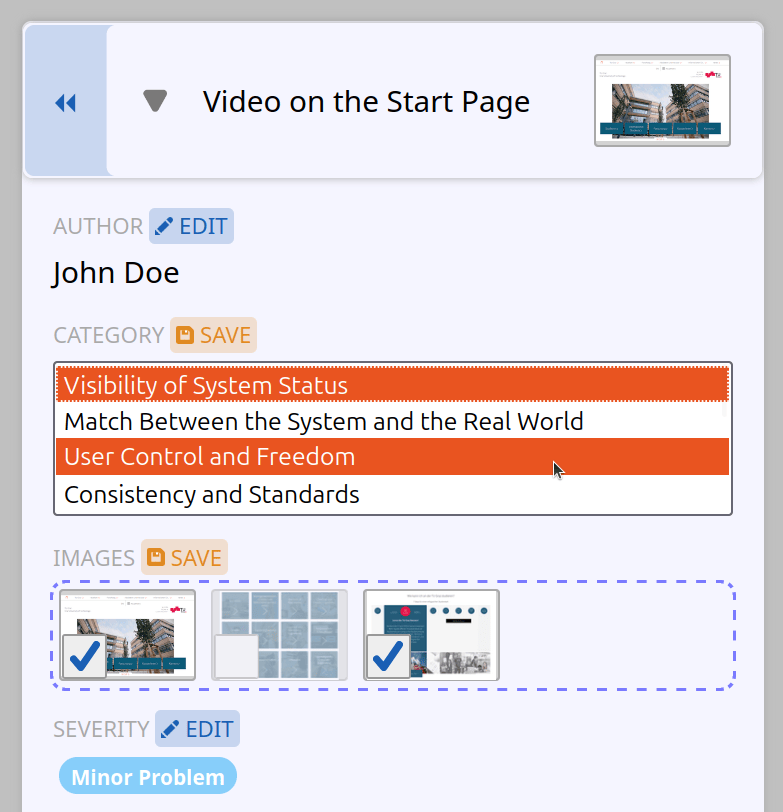
\includegraphics[frame,keepaspectratio,width=\linewidth,height=\halfh]
{images/edit-i.png}
\caption[Item Editing]{%
Properties can be made editable. A double click replaces the text with a
select box.
\imgcredit{Screenshot by Martin Rabensteiner.}
}
\label{fig:edit}
\end{figure}

\begin{figure}[tp]
\centering
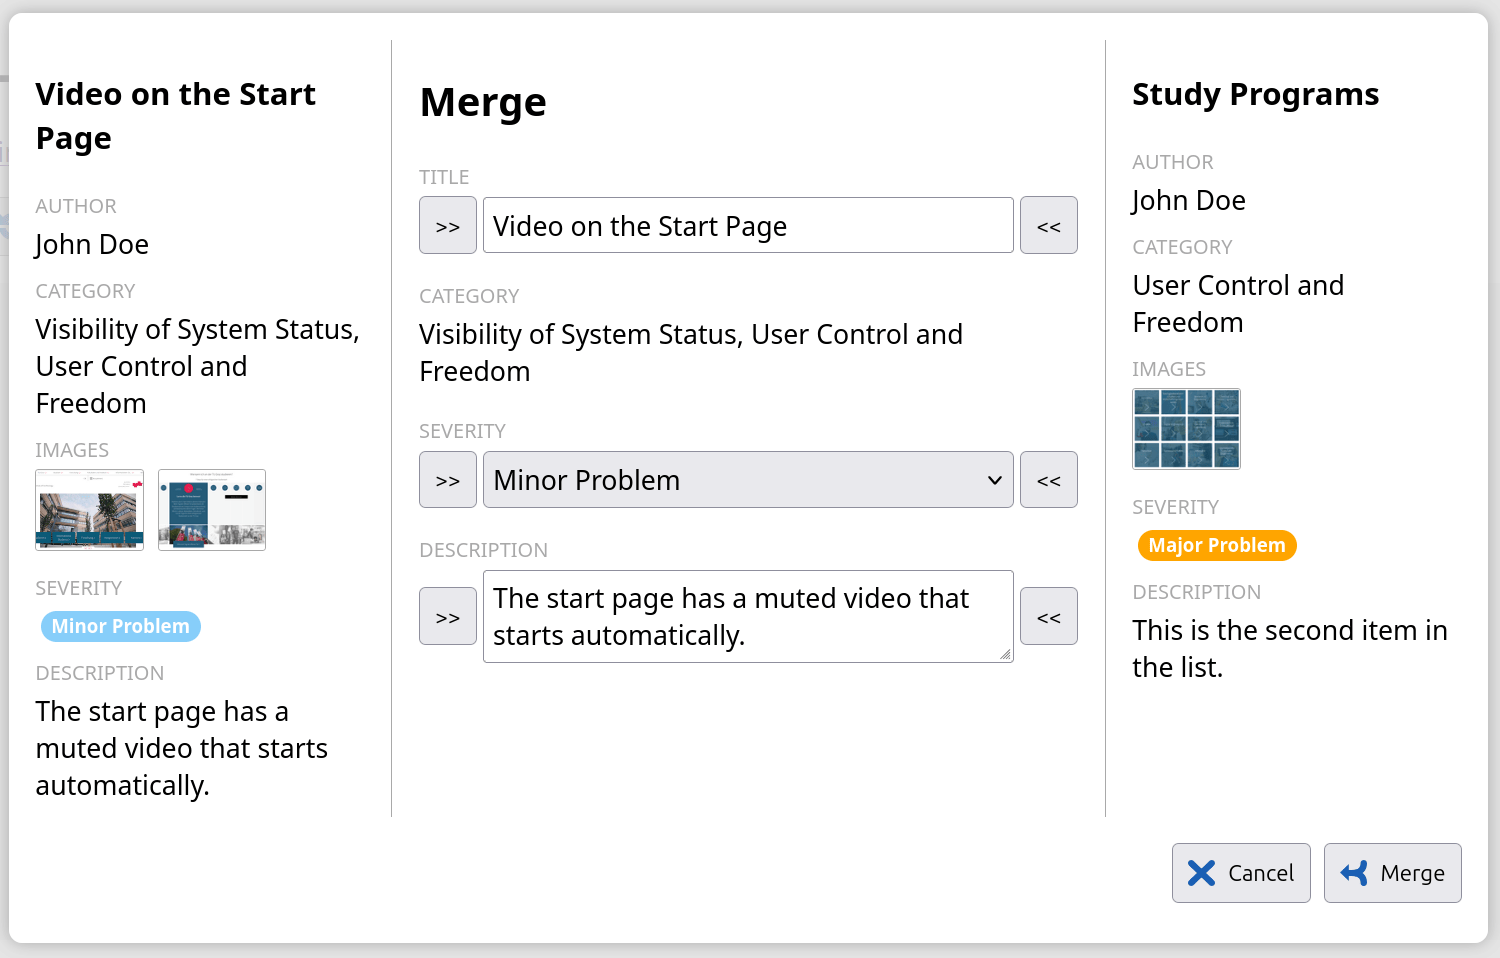
\includegraphics[frame,keepaspectratio,width=\linewidth,height=\halfh]
{images/merge-i.png}
\caption[Merge Item Window]{%
When merging two items, their properties are compared in a modal and can
be edited in the middle.
\imgcredit{Screenshot by Martin Rabensteiner.}
}
\label{fig:mergewindow}
\end{figure}

\begin{figure}[tp]
\centering
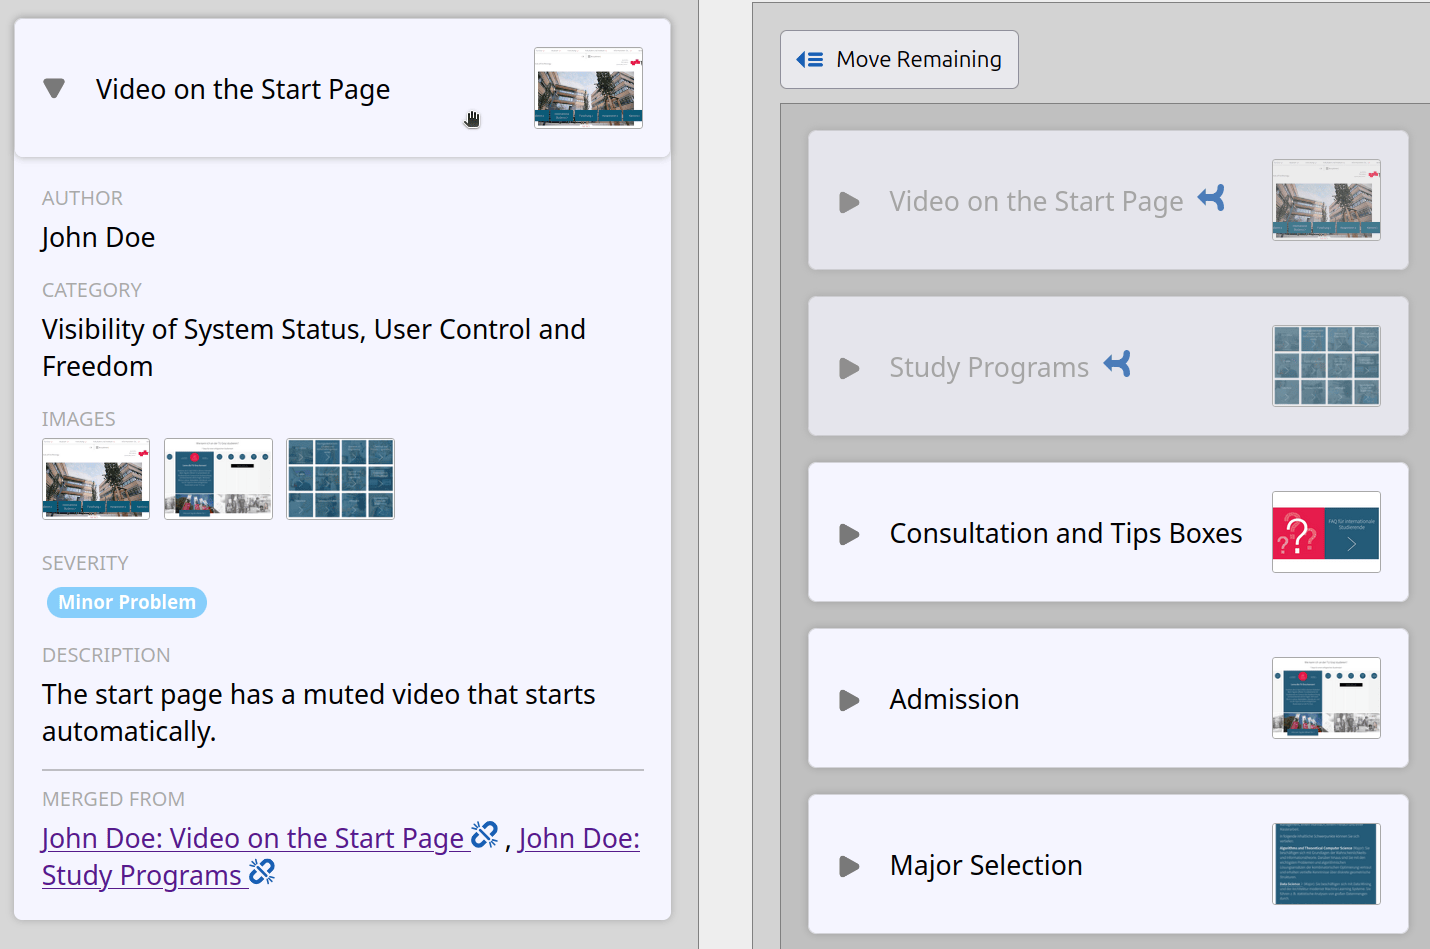
\includegraphics[frame,keepaspectratio,width=\linewidth,height=\halfh]
{images/merged-i.png}
\caption[Merged Item]{%
Merged items (right) appear greyed out and annotated with a merge icon.
The merge item (left) contains links to them.
\imgcredit{Screenshot by Martin Rabensteiner.}
}
\label{fig:mergeditems}
\end{figure}




\section{Items}
Items are created with a \elname{details} element. A classname and a
\cname{data-role} attribute are added from the predfined selectors. The inner part is defined by a template when initialising. All values that are defined for the item in the \vname{items} object can be used for rendering. Some values are added depending on the current state. These can be:
\begin{itemize}
  \item \vname{status}: Moved, merged or mergeitem.
  \item \vname{parent_id}: Contains the item's ID itself again, to be
    used in nested templates.
  \item \vname{mergedfrom}: Is a list of IDs from which the item is
    merged, applies only to mergeitems.
  \item \vname{mergedinto}: Contains the ID of the mergeitem, applies
    only to items that are merged.
  \item \vname{titleimg}: The first image that has an \vname{active}
    status that is not negative, applies only to items with images.
\end{itemize}




\section{User Actions and their implementations}

\subsection{Moving Items}
When items are moved to the mergelist, a clone of the regarding item is
produced.


\subsection{Editing Items}
The editing of items is not handed by the library directly, as this can
strongly depend on the individual implementation. Therefore, the
\vname{events.edit()} function can be called from the outside.


\subsection{Merging Items}
Merging is initiated by dragging one item over another in the mergelist.
A dialogue opens to compare the two items to merge, as seen in
Figure~\ref{fig:mergewindow}. The properties are shown to the left and
to the right. The middle column is for setting the properties of the
mergeitem. The properties of the left item are taken as default values.
Values can also be set or appended by clicking on the buttons left and
right to the fields. The items are only merged after clicking on the
\uiname{Merge} button. Original items are linked to the merge item and
vice versa. These connections can be detached.




\subsection{Detaching Items}
A detach button or link can be added to mergeitems or items that or
merged to loosen their connection. All attribute from the mergeitem stay
the same, except for the connection to the original item to detach. This
item then appears untouched in the origin list again. Two attributes
need to be set in order to execute the detach: \vname{data-from}
contains the ID of the original item, \vname{data-to} contains the ID of
the mergeitem.






\section{Icons}

Especially the merging icon made it necessary to work out custom icons
for this project. The icons were initially drafted in Inkscape and the
resulting SVG files manually revised and improved. All icons base on a
50x50 viewbox. Strokes have usually a width of 12 and a round linejoin.
All icons are listed in Table~\ref{tab:icons}. The iconset does not have
to be used, but can also be replaced or hidden completely. All items are
defined only in CSS stylesheets or templates and therefore not
obligatory for the library.


\newcommand{\iconbox}[1]{%
\includegraphics[margin=3mm,valign=m,width=6mm]{#1}
}%


\begin{table}[tp]
\tablerowstretch
\rowcolors{2}{}{tablerowcolour}
\centering
\begin{footnotesize}
\begin{tabularx}{\linewidth}
{>{\leavevmode\kern-\tabcolsep}llY<{\kern-\tabcolsep}}
\toprule
\textbf{Icon} & \textbf{Filename} & \textbf{Description} \\
\midrule
\iconbox{icons/caret.pdf} & \fname{caret.svg} & Replaces
the original triangle for \elname{details}. Indicates and controls its
open status. When opened, the icon is rotated 90 degrees.\\
%
\iconbox{icons/check.pdf} & \fname{check.svg} &
Used to indicate that an item is added to the mergelist, but not merged. \\
%
\iconbox{icons/close.pdf} & \fname{close.svg} &
For close buttons in dialogs. \\
%
\iconbox{icons/detach.pdf} & \fname{detach.svg} &
To detach items from mergeitems or the other way around.\\
%
\iconbox{icons/dragicon.pdf} & \fname{dragicon.svg} &
Used to rearranged items in the mergelist. Not included in the example.\\
%
\iconbox{icons/edit.pdf} & \fname{edit.svg} &
Button for editing values. \\
%
\iconbox{icons/merge.pdf} & \fname{merge.svg} &
Button to merge and also as indicator for items that are merged into another. \\
%
\iconbox{icons/move.pdf} & \fname{move.svg} &
For moving an item to the mergelist or back. \\
%
\iconbox{icons/moveall.pdf} & \fname{moveall.svg} &
Move all remaining items to the mergelist. \\
%
\iconbox{icons/openfile.pdf} & \fname{openfile.svg} &
Open a file as source for lists and items.\\
%
\iconbox{icons/redo.pdf} & \fname{redo.svg} &
History redo.\\
%
\iconbox{icons/save.pdf} & \fname{save.svg} & 
Save the current state of all lists. \\
%
\iconbox{icons/save_orange.pdf} & \fname{save_orange.svg} &
Save the current state of an item when editing.\\
%
\iconbox{icons/undo.pdf} & \fname{undo.svg} &
History undo.\\
\bottomrule
\end{tabularx}
\end{footnotesize}
\caption[Icons used in ListMerger]{%
Overview of icons made for and used within the library.}
\label{tab:icons}
\end{table}




\section{Challenges and Future Work}
\label{sec:challenges}
This section covers some noteworthy challenges during the development
process, that could not completely be satisfied, or just with some
workarounds, and further tasks.



\subsection{Cursor Behaviour when Dragging}
One useful feature idea was that the cursor is different when dragging
an item, depending on whether the item is approaching to be moved to the
mergelist (moving cursor) or merged into another item (adding cursor).
The \vname{event.datatransfer.dropEffect} property in JavaScript defines
the visual behaviour of the mouse cursor during a drag event
\parencite{mdn-dropeffect}. While the \vname{cursor} CSS property offers
a variety of 36 mouse cursors, in interaction with the operating system
\parencite{mdn-cursor}, this property is not taken into account as soon
as a drag event is started. The \vname{dropEffect} has offers a
selection of only four elements, all equivalent to options for the CSS
property (\vname{copy}, \vname{move}, \vname{link}, \vname{none}).

Mozilla Firefox does currently not support the change of the cursor, as
long as the concerning event listener is not changed. In the current
implementation, the event listener is the same for the mergelist and its
items. Otherwise, the event listener needs to be reassigned every time
an item is changed. Google Chrome does basically support the change
during an event, but at some points a \vname{none} cursor is wrongly
shown.

An alternative to the strict \vname{dropEffect} setting of drag events
is to rebuild the native drag-and-drop functionality with other mouse
events. Solutions like this, for example the one of
\textcite{gunduz-mouseover}, were considered and tried out, but did not
lead to sufficient results. This browser mechanics is known and
discussed throughout several discussions and issue reports in the web.
\parencite{chromium-cursorissue,horowitz-customizecursor} It should not
be ruled out that the ability to change the drop effect will eventually
be made easier by browser vendors in future.



\subsection{Flexbox Layout within display: contents}
In the examples, the whole page is nested in a flexbox grid
\parencite{mdn-flexbox}. All outer controls, titles, etc. are always
visible, and only the lists are scrollable. Due to the construction of
tabs with the \elname{details} tag, the CSS option {display: contents}
is used once to let the title be in row and the inner content only for
one list. This option shows only the inner part of the content and do
not produce a box by themselves \parencite{mdn-display}.

The outer box is removed, the flex bounding box is not valid any more,
and therefore the inner content scales to maximum, making the scrollbar
for the whole tab scope, and not just the inner part where the items
are. Furthermore, accessibility problems associated with this property
value are mentioned.

Different structures for HTML and CSS only tabs, like radio buttons and
lables \parencite{kliemann-radiotabs} were tried, but led to the same
problem. Eventually, a JavaScript ResizeObserver
\parencite{mdn-resizeobs} is introduced to monitor the tab height, and
adjust the inner lists height to it.


\subsection{Accessibility}
One of the main usability affordance of this project is to have a
drag-and-drop functionality. However, this is a functionality that is
not in line with accessibility affordance. Some features, like the
moving of items can already be done only by clicks, but others, like
merging or arranging can not. A possible implementation could be a
button for an accessibility, where buttons and menus for those actions
are shown additional next to items.

